\documentclass{article}
\usepackage{graphicx}
\usepackage[margin = 2cm]{geometry}
\usepackage{caption}
\usepackage{subcaption}

\title{PCO Laboratoire 5 \\
\large Modélisation par moniteur de Mesa}
\author{Benoît Delay, Eva Ray}

\begin{document}
\maketitle

\section*{Description des fonctionnalités du logiciel}

Le programme modélise une boutique de barbier. La boutique est constituée d'un salon dans lequel on trouve une salle d'attente avec
un nombre de siège fixes et une chaise de travail sur laquelle un client peut se faire couper les cheveux. Un certain nombre de clients
vont tenter de se faire couper les cheveux par le barbier. Le programme est doté d'une interface graphique, qui est animée grâce aux
annimations présentes dans la clase \texttt{PcoSalon} qui représentent les actions du barbier et des clients. \\

Les fonctionnalités du salon sont assez représentatives d'un salon de coiffure classique. Le salon est géré par un barbier qui s'occupe
de couper les cheveux des clients sur la chaise de travail. Lorsqu'il a fini de s'occuper d'un client, le barbier appelle le prochain client
parmi ceux qui sont en train d'attendre dans la salle d'attente. Le barbier fait bien attention à appeler les clients dans leur ordre
d'arrivée. S'il n'y a plus aucun client dans la salle d'attente, le barbier va faire une petite sieste et ne revient que lorsqu'un nouveau
client arrive à la porte de la boutique. Le comportement du barbier est simulé par la méthode \texttt{Barber::run()}. \\

Les clients, quant à eux, ont aussi un comportement prédéfini. Les clients qui souhaitent se faire couper les cheveux ne peuvent entrer
dans le salon que si celui-ci a assez de place pour les acueillir, c'est-à-dire s'il y a de la place dans la salle d'attente ou si aucun
client n'est présent dans le salon. Dans le second cas, la barbier est en train de faire une petite sieste, comme mentionné ci-dessus.
L'arrivée du nouveau client à la porte va réveiller le barbier qui se déplace jusqu'à la chaise de travail, où le nouveau client
va le rejoindre. Si le salon est plein, le
client va faire un petit tour avant de revenir voir si une place s'est libérée. Si le client accède à la salle d'attente, il va gentiment
s'asseoir sur une chaise libre et attend que le barbier l'appelle. Lorsque c'est le tour du client, il se dirige vers la chaise de travail,
où le barbier lui coupe les cheveux. Une fois la coupe finie, le client quitte le salon et attend que ses cheveux repoussent avant de
revenir se faire faire une nouvelle coupe. Le comportement d'un client est simulé par la méthode \texttt{Client::run()} \\

Les comportements décrits ci-dessus sont représentés par les méthodes de la clase \texttt{PcoSalon} et correspondent aux machines d'états
illustrées ci-dessous. \\

La terminaison du programme est gérée grâce aux méthodes \texttt{PcoSalon::endService()} et \\ \texttt{PcoSalon::isInService()}.
La fin du programme
est innitiée dès qu'une entrée utilisateur est déclenchée dans le terminal. Le salon est alors fermé. Les clients qui ne se trouvent pas
actuellement dans le salon rentrent chez eux. Le barbier finit de s'occuper de tous les clients qui sont encore dans le salon mais n'en
accepte pas de nouveau. Une fois qu'il a terminé son travail, il part dormir et termine sa journée. \\

Le logiciel simule le comportement du barbier et des clients par des threads différents, il est donc multi-threadé. Par conséquent, il doit 
assurer une bonne gestion de la concurrence pour les ressources partagées entre plusieurs threads. Les méthodes du salon sont ainsi implémentées 
à l'aide d'un moniteur de Mesa, qui permet de gérer la concurrence et les animations. 

\begin{figure}
    \centering
        \begin{subfigure}[b]{0.4\textwidth}
        \centering
        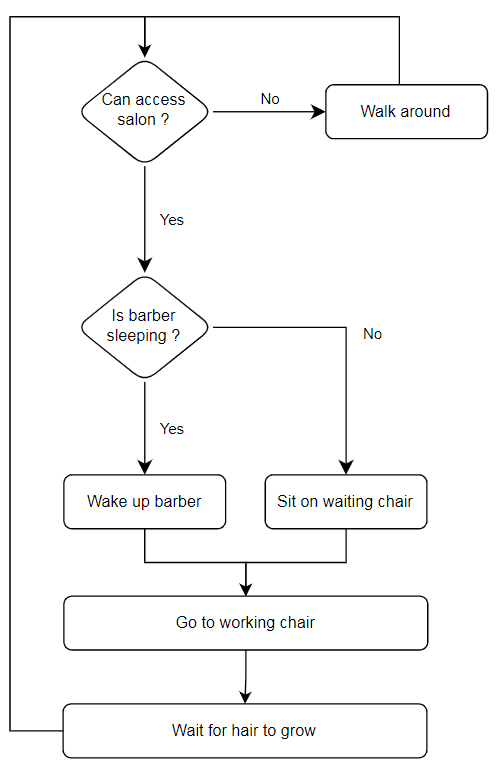
\includegraphics[width=\textwidth]{figures/machine_etat_client.png}
        \caption{Machine d'état du client}
        \label{fig:machine état client}
    \end{subfigure}
    \hfill
    \begin{subfigure}[b]{0.4\textwidth}
        \centering
        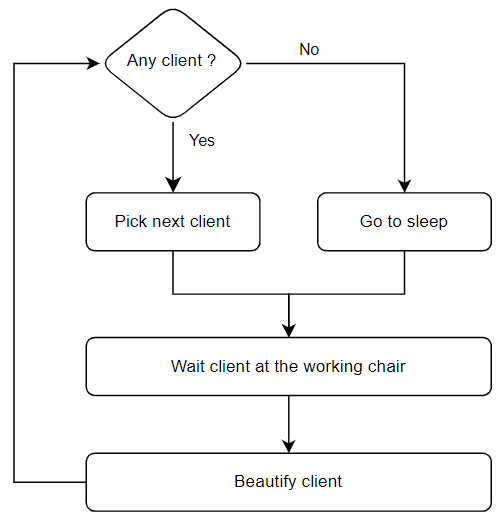
\includegraphics[width=\textwidth]{figures/machine_etat_barbier.png}
        \caption{Machine d'état du barbier}
        \label{fig:machine état barbier}
    \end{subfigure}
\end{figure}

\section*{Choix d'implémentation}
% Comment avez-vous abordé le problème, quels choix avez-vous fait, quelle 
% décomposition avez-vous choisie, quelles variables ont dû être protégées, ...

\subsection*{Variables de condition}

\section*{Tests effectués}
% Description de chaque test, et information sur le fait qu'il ait passé ou non

\section*{Conclusion}

\end{document}